\documentclass{article}
\usepackage[utf8]{inputenc}
\usepackage[top=2.5cm, bottom=2.5cm, left=2.5cm, right=2.5cm]{geometry}
\usepackage{amsmath}
\usepackage{amssymb}
\usepackage[bb=boondox]{mathalfa}
\usepackage{graphicx}
\usepackage{float}
\usepackage{parskip}
\setlength{\parindent}{0pt}
\usepackage[framed,numbered,autolinebreaks,useliterate]{mcode}

\usepackage{gensymb}

\author{Ahmed Hamdy Faramawy Mahmoud Shams El Din \\ hamdy@student.chalmers.se\\
Mohamed Takkoush\\
takkoush@student.chalmers.se}
\date{May 2019 }

\title{TME102 Vehicle dynamics advanced - Assignment 3}


\begin{document}

\maketitle

\section{Complete the vehicle model}
\subsection{Add equations of motion}
Equations of motion:

\begin{align*}
    \Dot v_x &= \frac{F_{3x} + F_{4x} + \left(F_{1x} + F_{2x}\right)\cdot     cos(\delta_f) - \left(F_{1y} + F_{2y}\right)\cdot                    sin(\delta_f)}{m} + r \cdot v_y\\
    \Dot v_y &= \frac{F_{3y} + F_{4y} + \left(F_{1y} + F_{2y}\right)\cdot     cos(\delta_f) + \left(F_{1x} + F_{2x}\right)\cdot                    sin(\delta_f)}{m} - r \cdot v_x\\
    \Dot r &= \frac{-l_2 \cdot \left(F_{3y} + F_{4y}\right)   +   l_1\cdot\left( \left(F_{1x} + F_{2x}\right)\cdot sin(\delta_f) + \left(F_{1y} + F_{2y}\right)\cdot cos(\delta_f) \right)}{I_{zz}}    \\ & + \frac{ \left( \frac{w}{2} \right)\cdot \left( 
F_{4x}-F_{3x} + \left( F_{2x}-F_{1x} \cdot cos(\delta_f) + \left( F_{1y}-F_{2y} \right)\cdot sin(\delta_f) \right)
\right)}{I_{zz}}
\end{align*}


\subsection{Add combined tyre slip}
Force limitation is applied in Matlab so that the longitudinal force for each tire does not exceed $\mu F_z cos(\alpha)$ or go below $-\mu F_z cos(\alpha)$. Then, $F_y$ for each tire is calculated based on the magic tire formula as follows:
\begin{align*}
    F_{y,max} &= \sqrt{(\mu F_z)^2-(F_x)^2}\\
    F_y &= F_{y,max} sin\left( C \cdot atan \left( B \alpha - E \left(B \alpha - atan \left(B \alpha \right)\right)\right)\right)
\end{align*}


\subsection{Test model }
\begin{figure}[H]
      \begin{minipage}[b]{0.5\linewidth}
      \centering
        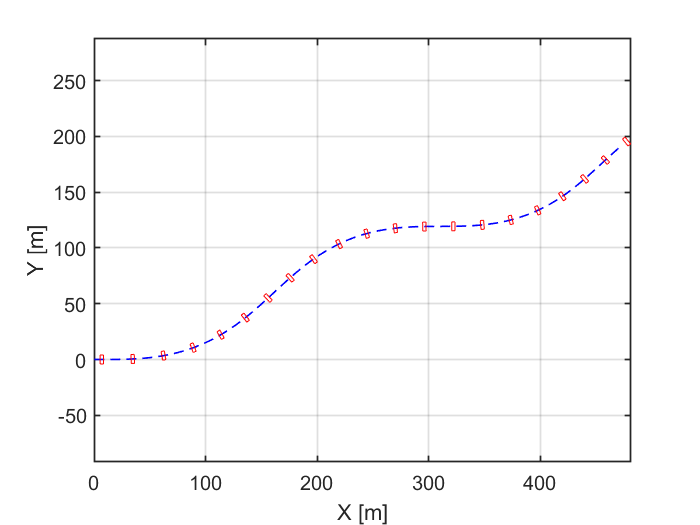
\includegraphics[width=\linewidth]{Figures/1_3_XY.png}
        %  \caption*{Trajectory} 
        % \label{fig:2_4_l}
    \end{minipage} 
    \begin{minipage}[b]{0.5\linewidth}
    \centering
        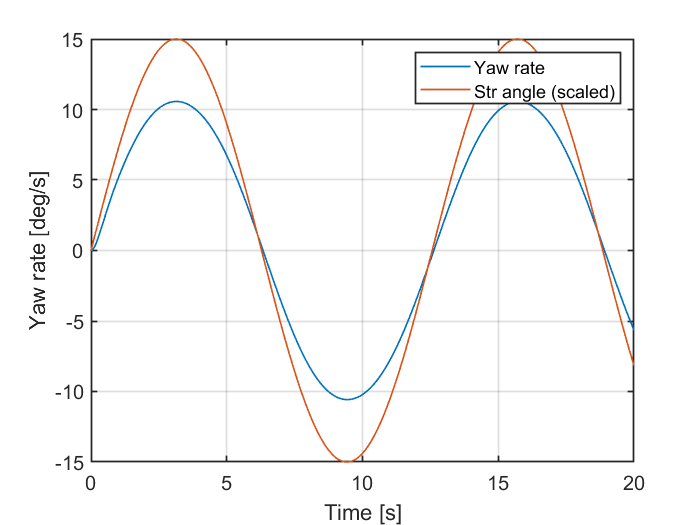
\includegraphics[width=\linewidth]{Figures/1_3_yaw.png}
        % \caption*{Yaw rate}
        % \label{fig:2_4_u}
    \end{minipage} 
    \caption{Base Vehicle Trajectory and Yaw rate for sine wave input}
    %  \label{fig:headbodyrelmotion}
\end{figure}

As seen in the figure above, the vehicle has a sine wave yaw rate, as expected. Since only the equations of motion are implemented, we shouldn't expect any phase shift in the response. And this is clear in the figure above where the peak yaw rate coincides with the peak steering angle input.


\subsection{Check stability in SWD}
For checking the stability of the vehicle, the sine with swell test is carried out in a loop format. The program will start from $60^{\circ}$ up until $300^{\circ}$ or until the vehicle fails one of the specified criteria. The base vehicle in this questions happens to pass all the tests, and hence it is a stable vehicle based on this test.

\section{Add load transfer}
\subsection{}
The provided equations for load transfer are applied on each wheel, with the respective sign convention. The roll stiffness and roll damping distributions are calculated respectively as follows:
\begin{align*}
    c_{\phi,1} &= c_{\phi} \cdot c_{\lambda}\\
    k_{\phi,1} &= k_{\phi} \cdot k_{\lambda}\\
\end{align*}

\subsection{Add roll dynamics}
The simulation is done in Simulink, and the results are in the next questions.

\subsection{Plot frequency response and coherence}
The following figures were obtained for the frequency sweep response with load transfer:

\begin{figure}[H]
    \centering
    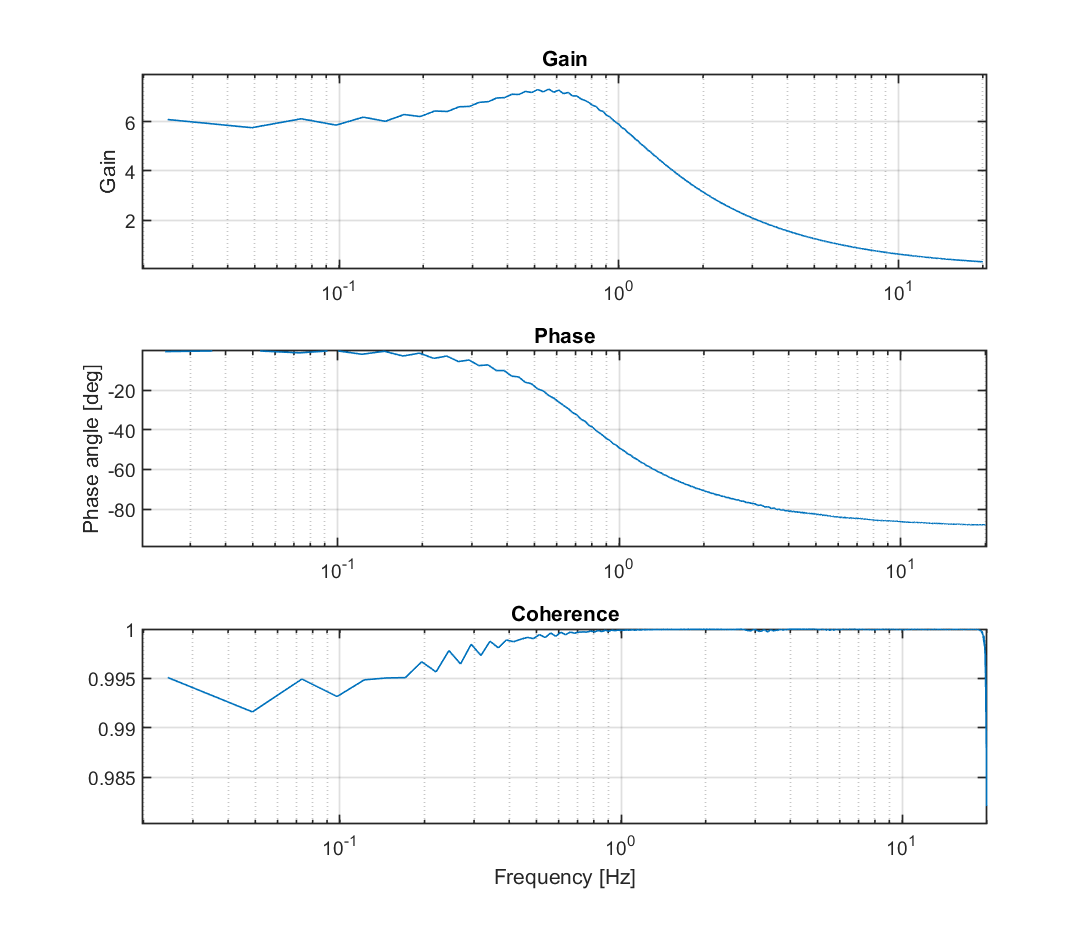
\includegraphics[width=0.8\textwidth]{Figures/2_3.png}
    \caption{Frequency Response of Vehicle with Load Transfer}
    % \label{fig:my_label}
\end{figure}

It can be seen in the figure above that the coherence of the transfer function is always above 0.99 in the whole range of frequencies up till $20Hz$. This means that the transfer function is reliable in all those frequencies, especially near the resonance frequency where the coherence is around 0.999.

\subsection{Determine resonance frequency}
It can be seen from the figure above, or from Matlab that the resonance frequency is at 0.6Hz (0.5615Hz). This is definitely close to the sine and dwell frequency of 0.7Hz by less than $\pm 0.3 Hz$.

This resonance frequency $(0.5615 Hz)$ will be used as the sine and dwell frequency throughout the report in order to achieve comparable results between the standard car, the ESC and the AARB.

\subsection{Test SWD with load transfer}
% fails both tests 1 and 2 at 140 degrees
\begin{figure}[H]
      \begin{minipage}[b]{0.49\linewidth}
      \centering
        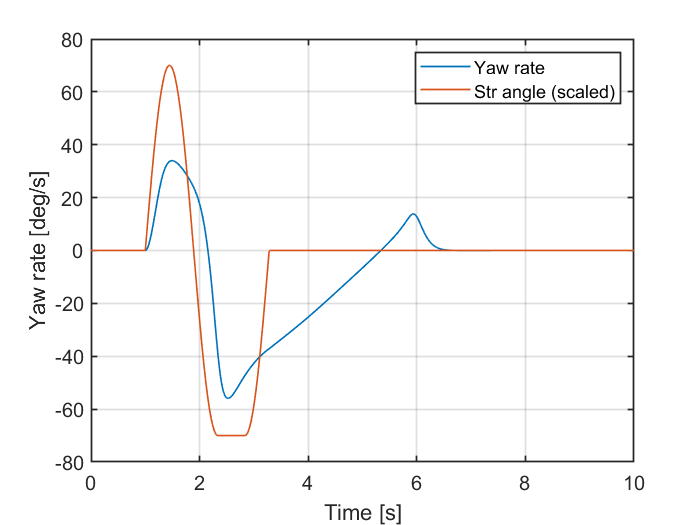
\includegraphics[width=\linewidth]{Figures/3_3_ESCoff.png}
        %  \caption*{Trajectory} 
        % \label{fig:2_4_l}
    \end{minipage} 
    \begin{minipage}[b]{0.49\linewidth}
    \centering
        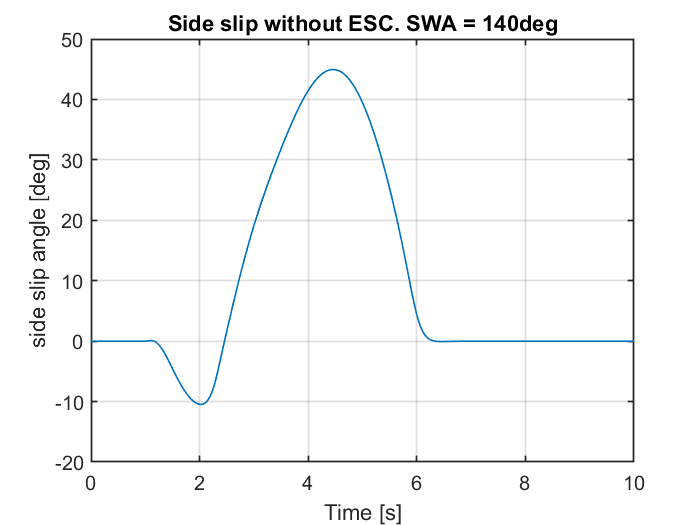
\includegraphics[width=\linewidth]{Figures/3_3_ESCoff_sideSlip.png}
        % \caption*{Yaw rate}
        % \label{fig:2_4_u}
    \end{minipage} 
    \caption{Side Slip and Yaw Rate with Load Transfer for Sine with Dwell Test}
    %  \label{fig:headbodyrelmotion}
\end{figure}

The figure above shows the simulation when the vehicle fails. The steering wheel input is $140^{\circ}$, and the vehicle fails the first and second test at the simultaneously. This means that the vehicle with load transfer is less stable than the ideal vehicle model. The reason is that upon adding load transfer, the forces on each side of the vehicle will increase or decrease respectively. This change in the $\Delta F$ will change the cornering stiffness of the vehicle and hence the handling characteristics. Generally, the cornering stiffness will increase on the outside wheels and decrease in the inside wheels due to the load transfer. However, because of the non-linearity of the tyres, the decrease is larger than the increase. Hence, the average cornering stiffness for one axle will decrease, giving the vehicle less grip. 

\section{Add brake based ESC}
\subsection{Determine reference yaw rate for ESC}

The steady state yaw rate gain for the bicycle model is expressed as the following:

\begin{equation}
    \frac{\omega}{\delta_f} = \frac{v_x}{L + K_u m v_x^2}
\end{equation}

This can be used to calculate reference yaw rate for a given vehicle speed $v_x$ and steering angle $\delta_f$. This reference is expressed as the following:

\begin{equation*}
    \omega_{ref,1} = \frac{v_x \delta_f}{L+K_u m v^2}
\end{equation*}

However, this does not take into account the maximum lateral force that the tyres can provide. This means that during the beginning of the maneuver, with a high steering angle $\delta_f$, the reference $\omega_{ref,1}$ is going too be to high. This could cause the system to induce oversteer as to increase the yaw rate, which would make the vehicle unstable during the beginning of the maneuver. 

Another limit is therefore needed to account for the maximum lateral force that the tyres can provide. Assuming that the maximum lateral force $Fy$ is provided. 

\begin{align*}
    \sum Fy = \sum F_z \mu_{0} & = \mu_0 mg = m a_y \Rightarrow  \\
    & a_{y,max} = \mu_0 g
\end{align*}

This can the be use to calculate the maximum available yaw rate as:

\begin{equation*}
    \omega_{ref,2} = \frac{a_{y,max}}{v_x} = \frac{\mu_0 g}{v_x} 
\end{equation*}

The final yaw rate reference $\omega_{ref}$ is then expressed as the signed minimum of these two. In matlab this was expressed as:

\begin{equation*}
    \omega_{ref} = sign(\omega_{ref,1})*min(|\omega_{ref,1}|,\omega_{ref,2})
\end{equation*}

This was evaluated in the upcoming questions, where $\omega_{ref}$ is plotted against the actual yaw rate. 

\subsection{Add the control algorithm for the ESC system}
In order to induce an oversteer or understeer, the ESC will brake on of the tires to create a moment around the center of gravity.
During a turn, if a car is oversteering, one of the outer wheels is braked. However, during an understeering situation, one of the inner wheels is braked by the ESC. To know which wheel to brake, front or rear, one has to look at the direction of the force and check which force has a longer moment arm.

\begin{figure}[H]
    \centering
    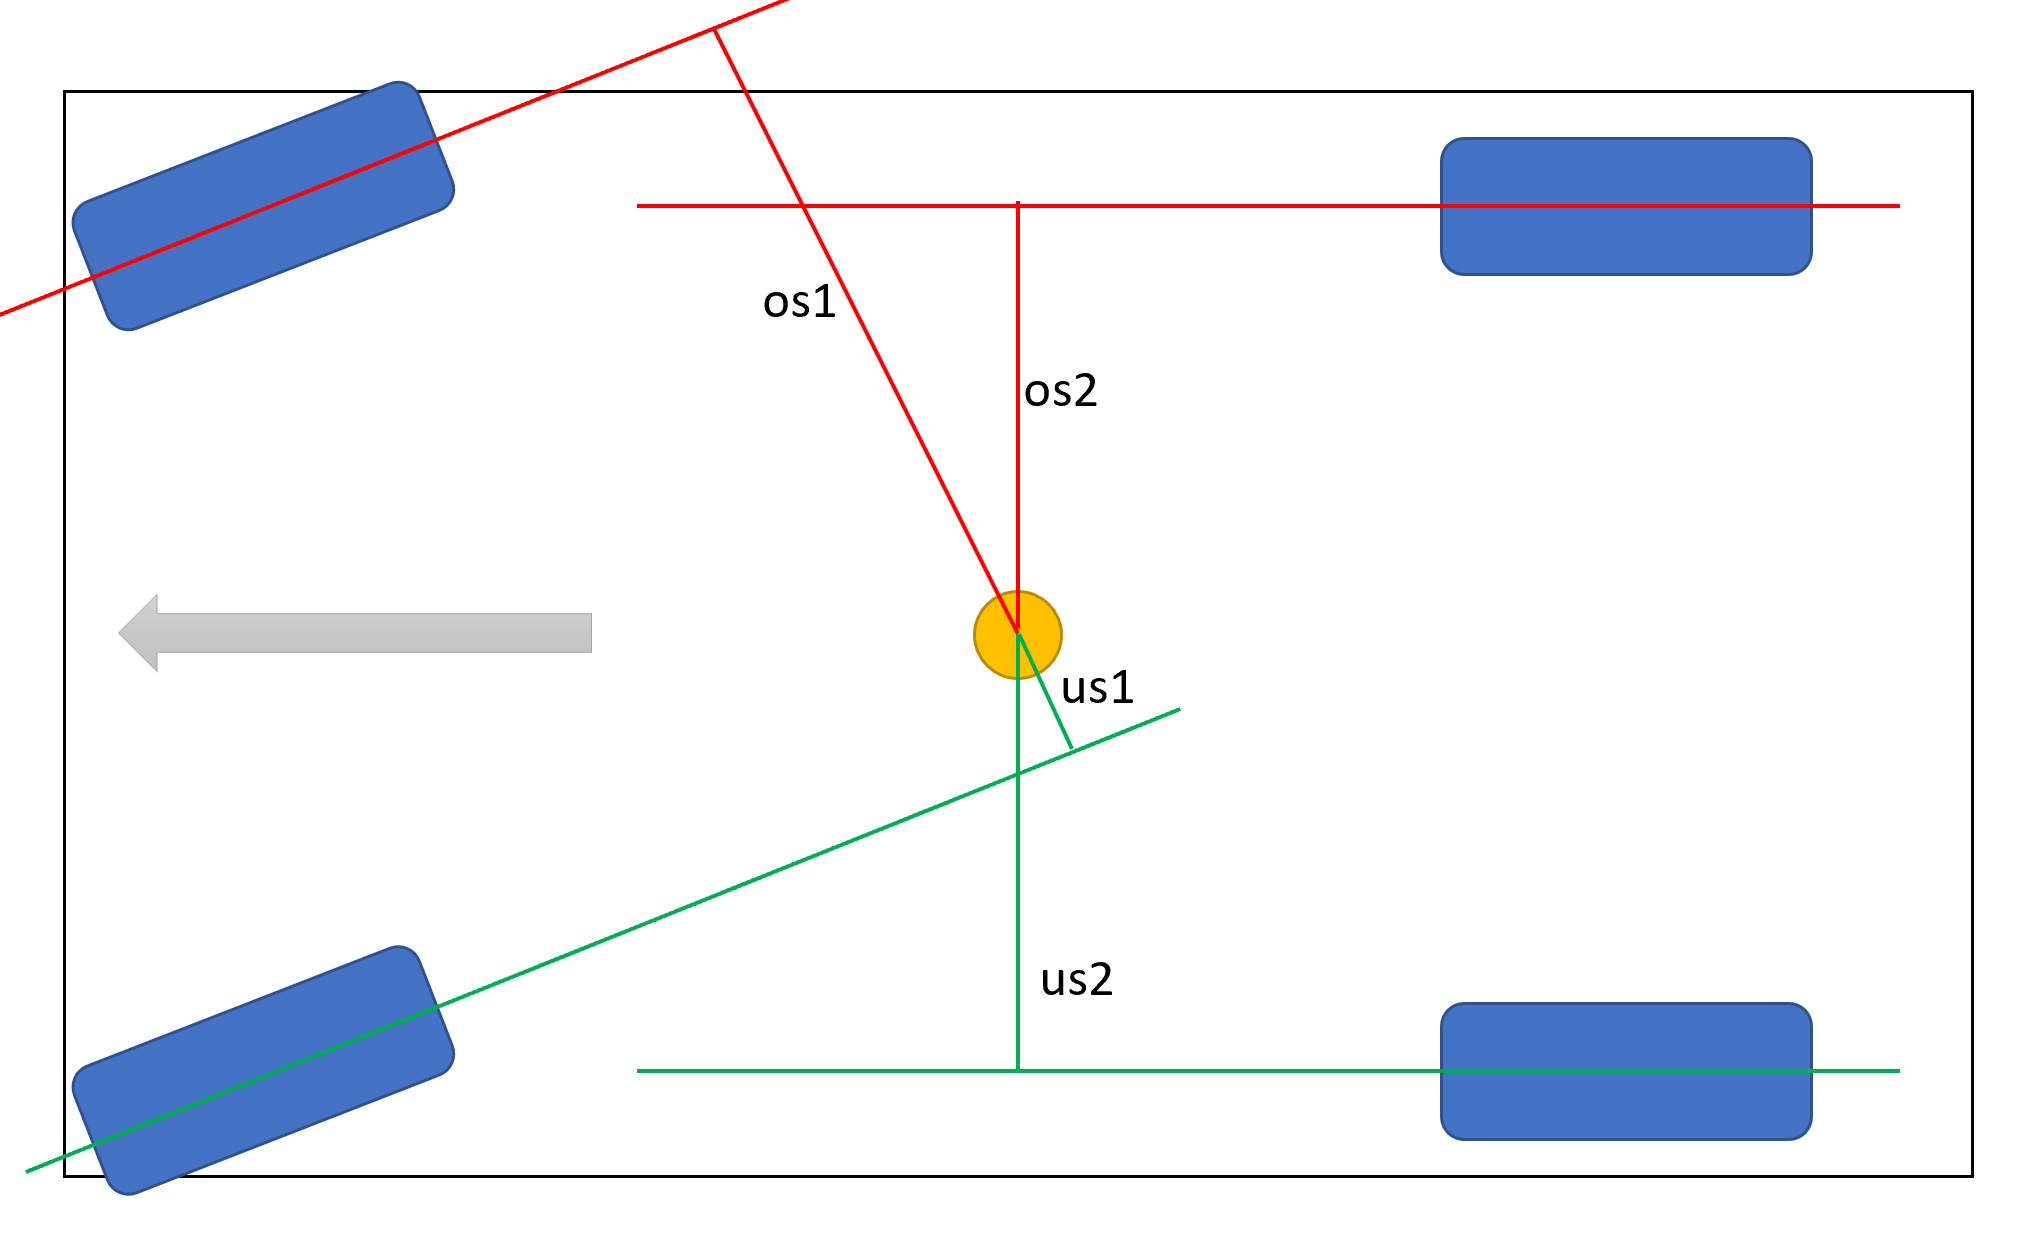
\includegraphics[width=0.7\textwidth]{Figures/underover.PNG}
    \caption{ESC Design Strategy}
    % \label{fig:my_label}
\end{figure}

By looking at the figure above, during oversteer, braking the front outer tire has a bigger moment arm compared to the rear wheel. This is the opposite for the understeer case where the moment arm of the force on the rear wheel is bigger than that on the front.

Hence the design is as follows:
\begin{itemize}
    \item Understeer: Brake inner rear wheel
    \item Oversteer: Brake outer front wheel
\end{itemize}

In Matlab, this algorithem was implemented as such, where $\omega =r$:

\begin{lstlisting}
 rErr = abs(r-rREF);

     FxReq = [0; 0; 0; 0;];
    if rErr > rErrLim && vx > uESCLim
        if abs(rREF) > abs(r)           % understeer
            if rREF > 0                 % left turn
                FxReq(3) = -escK*rErr;
            else                        % right turn
                FxReq(4) = -escK*rErr;
            end
        else                            % oversteer
            if rREF > 0                 % left turn
                FxReq(2) = -escK*rErr;
            else                        % right turn
                FxReq(1) = -escK*rErr;
            end
        end
    end
\end{lstlisting}

\subsection{Evaluate ESC performance and check side slip angle}

With the ESC enabled, the vehicle passed all the tests in the given region SWD $\in[60,300]\degree$. As to evaluate how it changes the vehicle's handling, a simulation was run with a steering angle of $140\degree$, since this is comparable with the base case. 

\begin{figure}[H]
      \begin{minipage}[b]{0.5\linewidth}
      \centering
        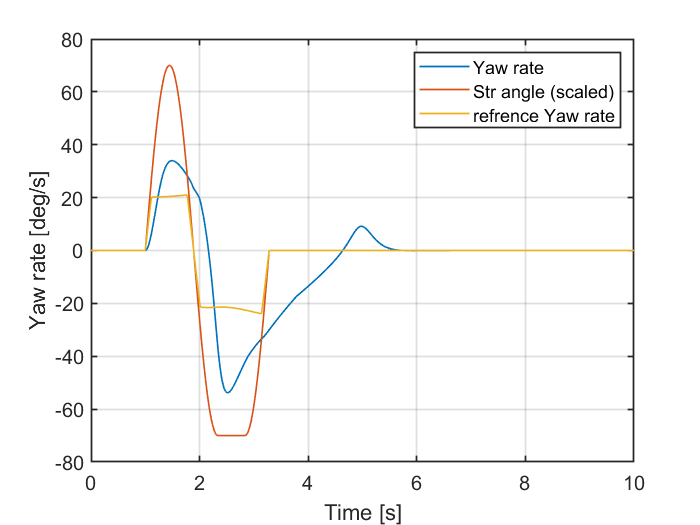
\includegraphics[width=\linewidth]{Figures/3_3_ESCon.png}
        %  \caption*{Trajectory} 
        % \label{fig:2_4_l}
    \end{minipage} 
    \begin{minipage}[b]{0.5\linewidth}
    \centering
        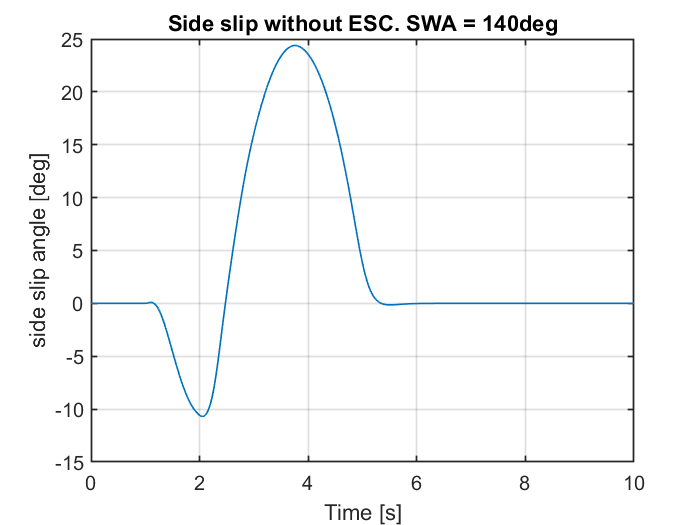
\includegraphics[width=\linewidth]{Figures/3_3_ESCon_sideSlip.png}
        % \caption{Yaw rate}
        % \label{fig:2_4_u}
    \end{minipage} 
    \caption{Side Slip and Yaw Rate with Load Transfer for Sine with Dwell Test with SWA 140\degree}
    %  \label{fig:headbodyrelmotion}
\end{figure}

As apparent by the figure above, side slip angle is lower than the case with ESC off and the yaw rate stabilises faster. This means that the vehicle is overall more stable and more responsive to steering input, even in transient motions. This would make the driver feel that the vehicle is more stable with ESC on, which is desirable.  



\section{Add active anti-roll bar algorithm}
\subsection{Explain how AARB affects handling}
Active anti-roll bars (AARB) are a a new trend on modern vehicles that is being used more often recently. The goal behind it is to decrease the rolling of the vehicle to improve ride comfort, but more importantly to improve the handling of the vehicle.
To do so, the AARB acts as if one added extra springs between the axle and the body. So the forces on the tires will be amplified (i.e. the outer tire, which is being pushed to the ground will be pushed even more, while the inner tire will be pulled up more). This might cause wheel lift in extreme cases, and the AARB should account for that.

When it comes to the comfort, an AARB decreasing roll of the passenger compartment during maneuvers will indeed improve the ride comfort of the passenger. Moreover, while normal driving on an uneven road, the vehicle will be change its rolling stiffness to maintain a smooth ride while going over imperfections on the road like bumps or potholes.

As for the handling, the AARB changes the roll stiffness of each axle independently to achieve the desired roll of the vehicle. If one considers one of the axles, increasing the roll stiffness will cause a higher load transfer between the left and right side of the vehicle. Due to the degenerative relation between $F_Z$ and the cornering stiffness in the tires, for the same $\Delta F_z$, the cornering stiffness of the inner tire will decrease more than the increase of the cornering stiffness of the outer tire. This will decrease the overall cornering stiffness of the axle. If the axle was in front, this will make the car more understeered. If the axle is in the back, the vehicle will become less understeered. By choosing  
a distribution between the front and rear stiffnesses, one can control the understeer gradient of the vehicle and change its handling characteristics.

\subsection{Implement AARB and reduce roll gradient to 70\%}

The AARB increases the stiffness on one axle by applying a torque that compresses the suspension on one side, and elongates it on the other. To increase the roll stiffness of the vehicle, the AARB should "push down" the outer tyres and "pull up" the inner. This increases the roll stiffness of the vehicle and reduces the body roll during cornering. 

To find the magnitude of the torque that needs to be applied, a moment balance is done about the RC point of the front and rear axles during steady state cornering. Steady state was assumed for simplicity.  

\begin{align*}
    0 &= \textbf{M} + (I_{xx}+m_sh^2)\ddot{\phi} + k \Dot{\phi} + C \phi_{ref} - mg\phi -a_ym_sh_0\\
      \text{Steady } & \text{state cornering} \Rightarrow \ddot{\phi} =\dot{\phi} =0 \\
    0 &= \textbf{M} + C \phi_{ref} - mg\alpha -a_ym_sh_0\\
    \text{Where}&\\
    \phi_{ref} &= 0.7\cdot rollGradient\cdot a_y \text{ (to reduce roll gradient to 70\%)}
\end{align*}

% In the previous equations, it is assumed that $\ddot{\phi} = \Dot{\phi}=0$  because of steady state assumption. 

It is to note out that the generated moment, in bold, is the torque added by the AARB. This torque has to counteract the moments caused by the center of gravity and the fictitious lateral acceleration about the roll center. On the other hand, the passive stiffness of the passive anti-roll bar and the suspension is aiding the AARB.

The equation uses $\phi_{ref}$ since the aim is to use the AARB to get rid of the difference between the desired and actual roll, while the suspension would take care of the rest.

% i removed the passive roll bar bit cuz we dont know if there is.

To evaluate performance of the AARB, two simulations, with the AARB on and off, were ran with a ramp maneuver. To avoid transient behaviour, the ramp had a slope of $0.5[\degree/s]$ and the simulation time extended to 100s. Then, the roll angel $\phi$ was plotted against the lateral acceleration $a_y$. The slope of this plot is the roll gradient of the vehicle. As recommended by the teacher, this should be evaluated for lateral accelerations between $2-4[m/s^2]$. The results are shown below. 

\begin{figure}[H]
      \begin{minipage}[b]{0.49\linewidth}
      \centering
        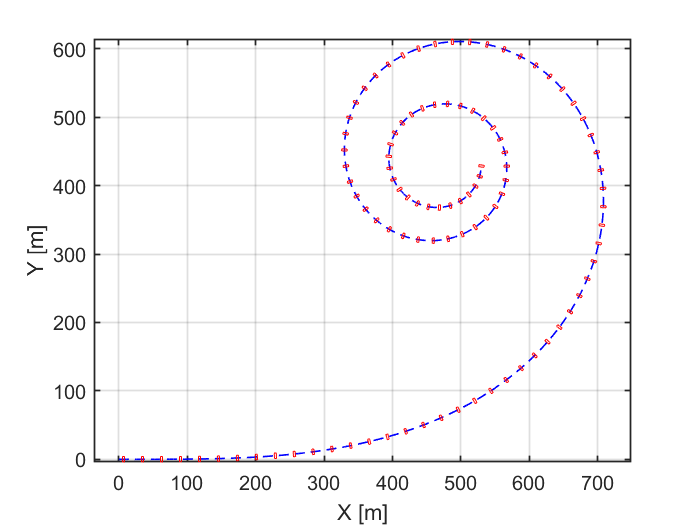
\includegraphics[width=\linewidth]{Figures/4_2_path.png}
        %  \caption*{Trajectory} 
        % \label{fig:2_4_l}
    \end{minipage} 
    \begin{minipage}[b]{0.49\linewidth}
    \centering
        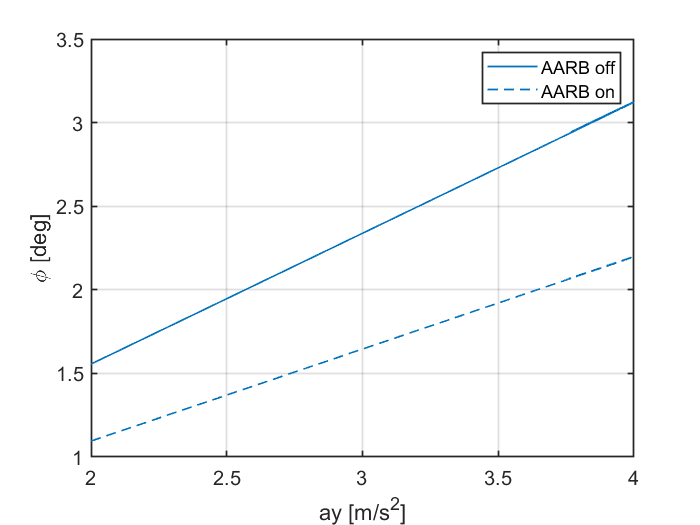
\includegraphics[width=\linewidth]{Figures/4_2_rollGrad.png}
        % \caption*{Yaw rate}
        % \label{fig:2_4_u}
    \end{minipage} 
    \caption{Path and Roll Gradient Comparison for a ramp steer input}
    %  \label{fig:headbodyrelmotion}
\end{figure}

\begin{figure}[H]
    \centering
    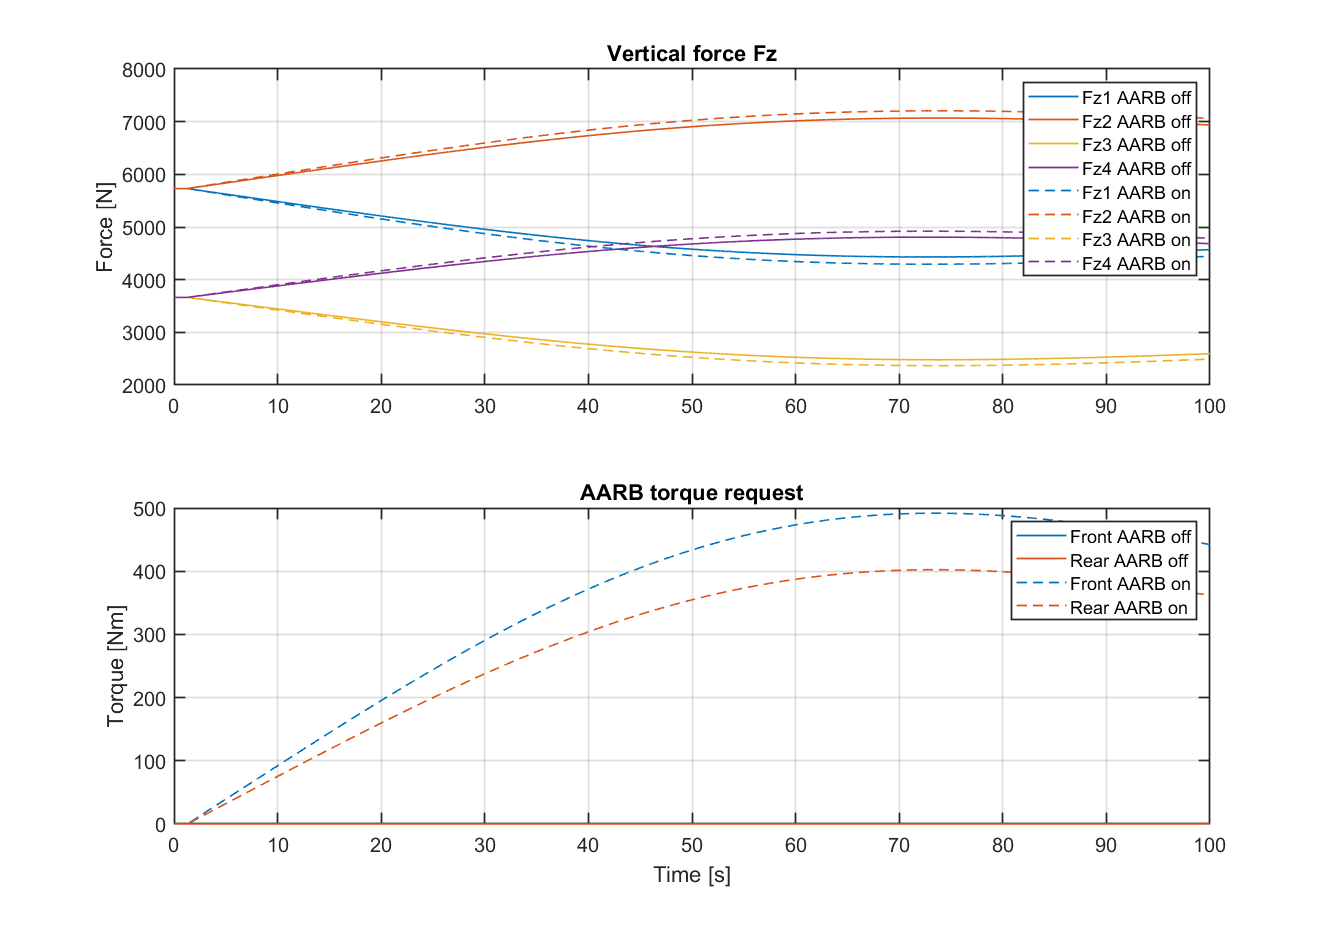
\includegraphics[width = \textwidth]{Figures/4_2_Fz.png}
    \caption{Tire Forces and required AARB torques}
    % \label{fig:my_label}
\end{figure}

\begin{table}[H]
    \centering
    \begin{tabular}{c|l}
         & Roll gradient $[\degree/(m/s^2)]$ \\\hline
        AARB off & 0.7850 \\
        AARB on &   0.5521 (70.33\%)
    \end{tabular}
    \caption{Roll gradient values}
    \label{tab:my_label}
\end{table}

As shown by the table above, the AARB seceded to bring the roll gradient of the vehicle to near $70\%$ of the original value. To test if this control method works for other percentages, it was tested for $50\%$ and $60\%$ as well and it produces similar results ($50\%$ and $60\%$ $\pm 0.4\%$). The small error might be due to $\ddot{\phi}$ and $\dot{\phi}$ not actually being 0. The non-linearity of the tyres might also have had an affect. 

\subsection{How can AARB affect transient behaviour}

As discussed before, changing the stiffness of the front and rear axles can make the vehicle more or less understeer. In the simulation, This was achived by changing the roll stiffness distribution $\lambda_c\phi$. To test this, three  simulations , AARB off, AARB induced understeer and AARB induced oversteer, were run with a step steer of $140\degree$ amplitude.  The resuts are shown below.

\begin{table}[H]
    \centering
    \begin{tabular}{c|c|c}
                    & understeer & oversteer\\\hline
         $\lambda_{c\phi}$ & 1.1  & -0.1\\
          $c_{\phi f}$ & $c_\phi\lambda_c$ & 0\\
          $c_{\phi r}$ & 0 &$c_\phi(1-\lambda_{c\phi})$
    \end{tabular}
    \caption{Controller input parameters for understeer and oversteer}
    \label{tab:my_label}
\end{table}

The parameters in the table above were, due to time constraints, found via trial and error until the required handling behaviour was achieved. 

\begin{figure}[H]
\begin{minipage}[b]{0.49\linewidth}
    \centering
    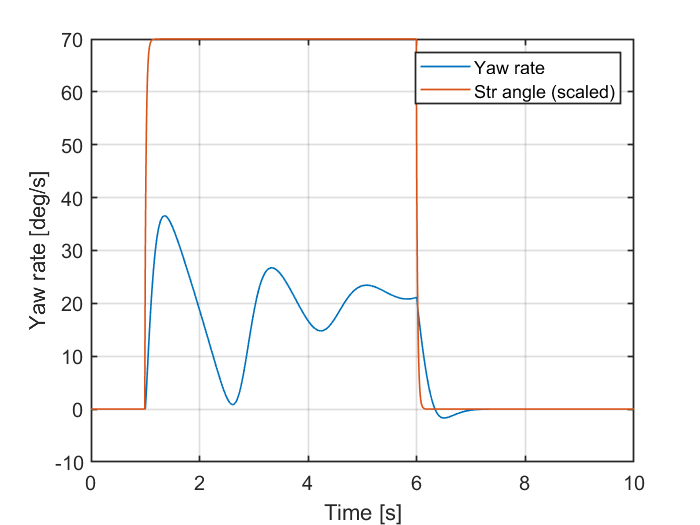
\includegraphics[width = \textwidth]{Figures/4_3_normal_140.png}
    \caption{AARB off}
\end{minipage}
\begin{minipage}[b]{0.49\linewidth}
    \centering
    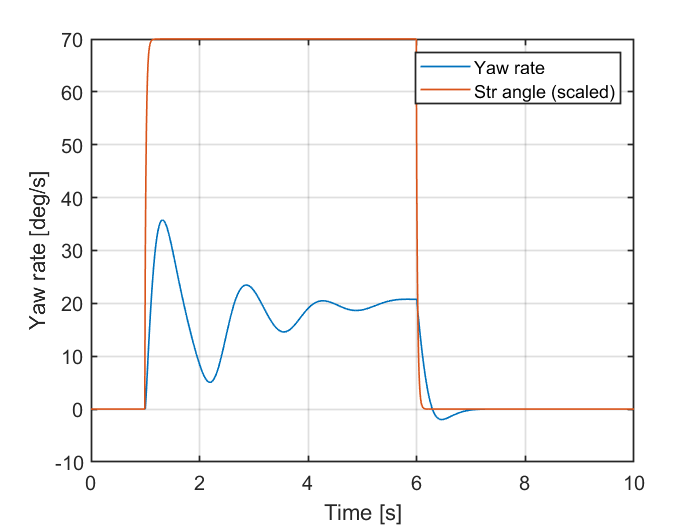
\includegraphics[width = \textwidth]{Figures/4_3_understeer_140.png}
    \caption{AARB induced understeer}
\end{minipage}
\begin{minipage}[b]{\linewidth}
    \centering
    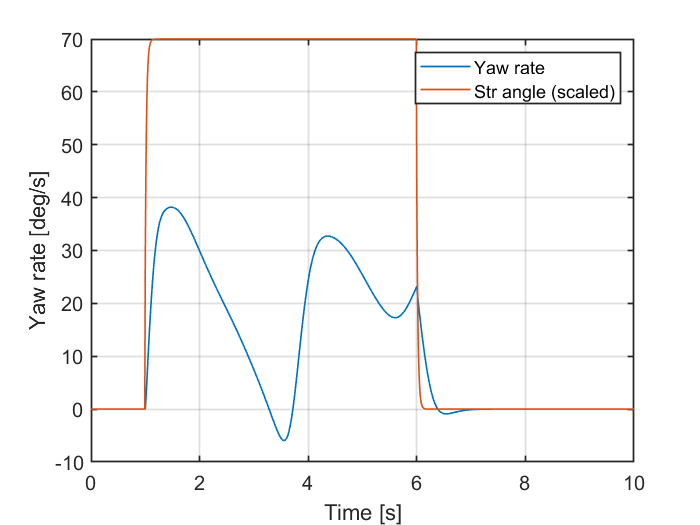
\includegraphics[width = 0.49 \textwidth]{Figures/4_3_oversteer_140.png}
    \caption{AARB induced oversteer}
\end{minipage}
\caption{Three simulations for step steer with 140$\degree$ amplitude}
\end{figure}

As can be seen in the figures above, the understeer case stabilises fastest. Moreover, the over steer case actually reaches a negative yaw rate for a positive steering angle and takes longer to stabilise. 

\subsection{Make vehicle understeer in SWD maneuver}

The same controller found in the task above was used here with for the SWD maneuver with the steering amplitude range SWD $\in[60,300]\degree$. The results were that the vehicle passed the test for the entire range. To see how the behaviour has changed, a simulation was run for steering amplitude $140\degree$ with the results shown below. 

\begin{figure}[H]
\begin{minipage}[b]{0.49\linewidth}
    \centering
    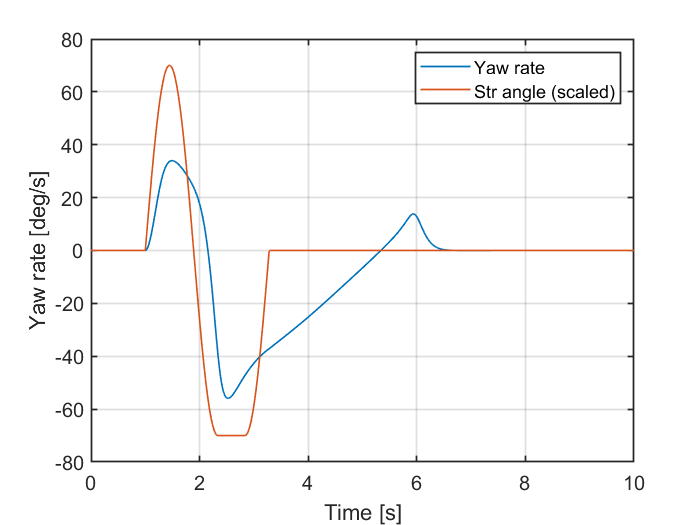
\includegraphics[width=\textwidth]{Figures/4_4_yaw_normalSteer_140deg.png}
    \caption{AARB off}
    \label{fig:my_label}
\end{minipage}
\begin{minipage}[b]{0.49\linewidth}
    \centering
    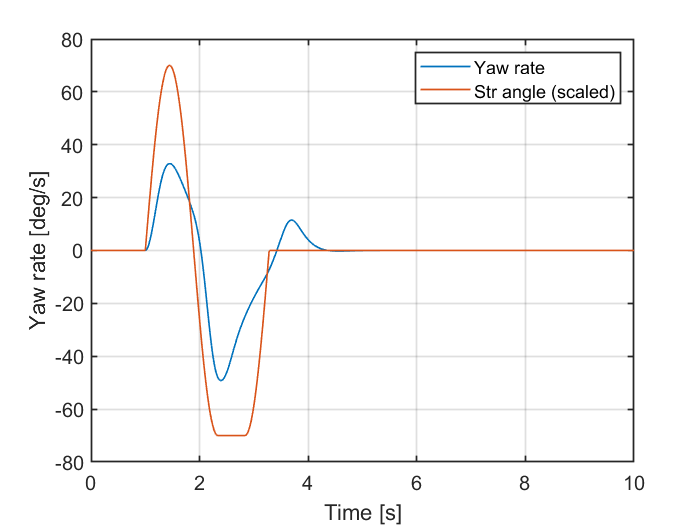
\includegraphics[width=\textwidth]{Figures/4_4_yaw_underSteer_140deg.png}
    \caption{AARB induced understeer}
    \label{fig:my_label}
\end{minipage}
\begin{minipage}[b]{0.9\linewidth}
    \centering
    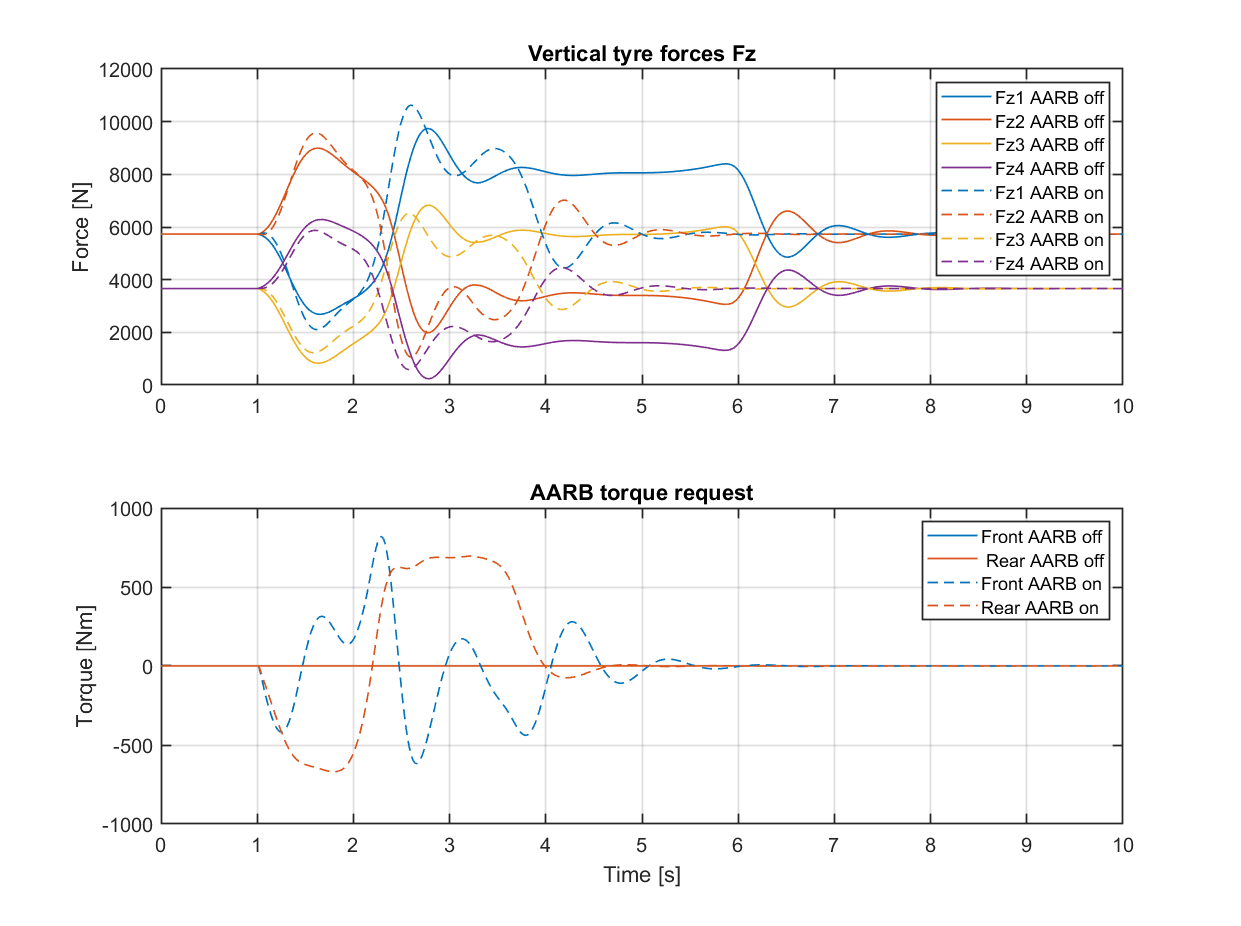
\includegraphics[width=\textwidth]{Figures/4_4_Fx_MxReq.png}
    \caption{Comparison between tyre forces for SWD with steering amplitude 140$\degree$}
\end{minipage}
\end{figure}

As seen above, the AARB makes the vehicle more stable through inducing understeer. This is apparent as the yaw rate returns to 0, and the vertical tyre forces stabilise, faster than with AARB off. 





\newpage
\section{MatlabCode}
\begin{lstlisting}
%% Question 1 
%% 1.3 test the model with sine wave steering 0.6 Hz and 30deg steering 

clear all;
run('initModel')

u0 = 100/3.6;
manoeuver = 5; % Sine wave 30deg 0.5Hz
makePlots = 1; 
simTime = 20;

run('runSimulation.m')
%% 1.4 Speed of 100km/h with different steering until fail

clear all;
run('initModel')

u0 = 100/3.6;

manoeuver = 3;
loadTrans = 0;

testAmplitudes = 60:5:300; %deg

for i2 = 1:length(testAmplitudes)
    strAmpSWD = testAmplitudes(i2);
    run('runSimulation');
    if TestsPass == 0
        strAmpSWD
        break
    end
end

run('postFcn.m')
%% Question 2
%% 2.1 complete equations 
%% 2.2 and 2.3 simulation with 10deg steering, sweep upto 20Hz

clear;
run('initModel')


u0 = 100/3.6;

strAmpSS    = 10;
strMaxFreq  = 20; 

manoeuver = 2; % sweep manouever 
loadTrans = 1;
simTime     = 100;

run('runSimulation');


fs=1/sampleTime;
[tf,f] = tfestimate(deltaf,r,[],[],[],fs);
gain = abs(tf);
phase = rad2deg(angle(tf));
coherence = mscohere(deltaf,r);

idx_f = find(f>0 & f<20);

figure(1);
subplot(3,1,1)
semilogx(f(idx_f),gain(idx_f)); grid on
title('Gain')
ylabel('Gain')

subplot(3,1,2)
semilogx(f(idx_f),phase(idx_f)); grid on
title('Phase')
ylabel('Phase angle [deg]')

subplot(3,1,3)
semilogx(f(idx_f),coherence(idx_f)); grid on
title('Coherence')
xlabel('Frequency [Hz]')
% 2.4  Gain and natural frequency
[maxGain, maxGain_i] = max(gain(idx_f)); % 
ResonanceFreq = f(idx_f(maxGain_i)); % the resonance frequency 
%% 2.5 Speed of 100kmh with differnt steering until fail with load transfer

clear;
run('initModel')

manoeuver = 3; % SWD
loadTrans = 1;
strFreq     =  0.5615; % changed to resonance 0.7 % This frequency is from the NHTSA ESC test specifications. 
SWDend      = 1/strFreq+dwell+tStart;
SWDduration = 1/strFreq+0.5;

testAmplitudes = 60:5:300; %deg

for i2 = 1:length(testAmplitudes)
    strAmpSWD = testAmplitudes(i2);
    run('runSimulation');
    if TestsPass == 0
        strAmpSWD
        break
    end
end

run('postFcn.m')

% plot side slip 

figure;
plot(t,rad2deg(v./u)); grid on
title('Side slip without ESC. SWA = 140deg')
xlabel('Time [s]')
ylabel('side slip angle [deg]')

% 140 degs 
%% Question 3
%% 3.1, 3.2 and 3.3 Testing limits for ESC 

clear;
run('initModel')

manoeuver = 3; % sweep manouever 
loadTrans = 1;
makePlots = 0;
strFreq     =  0.5615; % changed to resonance 0.7 % This frequency is from the NHTSA ESC test specifications. 
SWDend      = 1/strFreq+dwell+tStart;
SWDduration = 1/strFreq+0.5;

testAmplitudes = 60:5:140; %deg

ESC = 1;

for i2 = 1:length(testAmplitudes)
    strAmpSWD = testAmplitudes(i2);
    run('runSimulation');
    if TestsPass == 0
        strAmpSWD
        break
    end
end

% plot side slip
figure;
plot(t,rad2deg(v./u)); grid on
title('Side slip without ESC. SWA = 140deg')
xlabel('Time [s]')
ylabel('side slip angle [deg]')
%% Question 4 
%% 4.1 completed equations in the simulink 
%% 4.2  Evaluating the body roll gradient

clear;
run('initModel')

manoeuver = 1; % Ramp
loadTrans = 1;
makePlots = 0;
simTime = 100;



run('runSimulation');

idx_ay = find(abs(ay)>2 & abs(ay)<4);

figure(2);
title('Roll Gradient')
set(gca,'ColorOrderIndex',1);
plot(ay(idx_ay),rad2deg(phi(idx_ay))); grid on; hold on
xlabel('ay [m/s^2]')
ylabel('\phi [deg]')

figure(3)
subplot(2,1,1)
set(gca,'ColorOrderIndex',1);
plot(t,Fz); hold on
subplot(2,1,2)
set(gca,'ColorOrderIndex',1);
plot(t,MxReq); hold on


rollGradient = (phi(idx_ay(1))-phi(idx_ay(end)))/(ay(idx_ay(1))-ay(idx_ay(end)));

% rollGradient =
% 
%     0.0137
%%  4.2 AARB reducing rollgradient to 70%

clear;
run('initModel')

manoeuver = 1; % Ramp
loadTrans = 1;
makePlots = 0;
simTime = 100;
rollGradient =  0.0137;
rollGrad_70 = 1;

AARB = 1;

run('runSimulation');

idx_ay = find(abs(ay)>2 & abs(ay)<4);

figure(2);
set(gca,'ColorOrderIndex',1);
plot(ay(idx_ay),rad2deg(phi(idx_ay)),'--'); grid on; hold on
xlabel('ay [m/s^2]')
ylabel('\phi [deg]')
legend('AARB off', 'AARB on')

rollGradient2 = (phi(idx_ay(1))-phi(idx_ay(end)))/(ay(idx_ay(1))-ay(idx_ay(end)));

figure(3)
subplot(2,1,1)
set(gca,'ColorOrderIndex',1);
plot(t,Fz,'--'); hold on; grid on 
title('Vertical force Fz')
ylabel('Force [N]')
legend('Fz1 AARB off','Fz2 AARB off','Fz3 AARB off','Fz4 AARB off', ... 
    'Fz1 AARB on','Fz2 AARB on','Fz3 AARB on','Fz4 AARB on')

subplot(2,1,2)
set(gca,'ColorOrderIndex',1);
plot(t,MxReq,'--'); hold on; grid on
title('AARB torque request')
legend('Front AARB off', 'Rear AARB off', 'Front AARB on', 'Rear AARB on' )
ylabel('Torque [Nm]')
xlabel('Time [s]')

PercentageDiff = rollGradient2/rollGradient;
%% 4.3 Testing step steer and release 

clear;
run('initModel')

manoeuver = 4; % Step and release
loadTrans = 1;
make_understeer = 1; % 0 = is normal, 1 more understeer, -1 less understeer
makePlots = 1;
simTime = 10;
strAmpSS = 140;
rollGradient =  0.0137;

for i2 =1:2
    AARB = 3-i2; % first without anti roll bar then with
    run('runSimulation');
    
    idx_ay = 1:1:length(ay);%find(abs(ay)>2 & abs(ay)<4);

    if i2 == 1
        lineType = '-';
    else
        lineType = '--';
    end

    figure(4)%'Name','Rollgradient');
    set(gca,'ColorOrderIndex',1);
    plot(ay(idx_ay),rad2deg(phi(idx_ay)),lineType); grid on; hold on
    xlabel('ay [m/s^2]')
    ylabel('\phi [deg]')
    
    rollGradient2 = (phi(idx_ay(1))-phi(idx_ay(end)))/(ay(idx_ay(1))-ay(idx_ay(end)));
    
    figure(5)%'Name','Forces')
    subplot(2,1,1)
    set(gca,'ColorOrderIndex',1)
    plot(t,Fz,lineType); hold on; grid on;
    subplot(2,1,2)
    set(gca,'ColorOrderIndex',1)
    plot(t,MxReq,lineType); hold on; grid on;
    
%     figure(6)%'Name','slips',)
%     subplot(1,2,1)
%     set(gca,'ColorOrderIndex',1)
%     plot(alpha(:,1), Fy(:,1), lineType); hold on; grid on;
%     plot(alpha(:,2), Fy(:,2), lineType); hold on;
%     subplot(1,2,2)
%     set(gca,'ColorOrderIndex',1)
%     plot(alpha(:,3), Fy(:,3), lineType); hold on; grid on;
%     plot(alpha(:,4), Fy(:,4), lineType); hold on;q
end

figure(4)
title('Vehicle roll')
legend('AARB off', 'AARB on')

figure(5)
subplot(2,1,1)
title('Vertical tyre forces Fz')
ylabel('Force [N]')
legend('Fz1 AARB off','Fz2 AARB off','Fz3 AARB off','Fz4 AARB off', ...
    'Fz1 AARB on','Fz2 AARB on','Fz3 AARB on','Fz4 AARB on')
subplot(2,1,2)
title('AARB torque request')
xlabel('Time [s]')
ylabel('Torque [Nm]')
legend('Front AARB off', ' Rear AARB off', 'Front AARB on', 'Rear AARB on')
%% 4.4 making the vehicle understeer with the AARB

clear;
run('initModel')

strFreq     =  0.5615; % changed to resonance 0.7 % This frequency is from the NHTSA ESC test specifications. 
SWDend      = 1/strFreq+dwell+tStart;
SWDduration = 1/strFreq+0.5;

manoeuver = 3; % sine with dwell 
loadTrans = 1;
makePlots = 1;
simTime = 10;
rollGradient =  0.0137;
make_understeer = 1;

strAmpSWD = 140;

for i2 =1:2
    AARB = 3-i2; % first without anti roll bar then with
    run('runSimulation');
    
    idx_ay = 1:1:length(ay);%find(abs(ay)>2 & abs(ay)<4);

    if i2 == 1
        lineType = '-';
    else
        lineType = '--';
    end
    
%     figure(12)%'Name','Rollgradient');
%     plot(ay(idx_ay),rad2deg(phi(idx_ay)),lineType); grid on; hold on
%     xlabel('ay [m/s^2]')
%     ylabel('\phi [deg]')
%     
%     rollGradient2 = (phi(idx_ay(1))-phi(idx_ay(end)))/(ay(idx_ay(1))-ay(idx_ay(end)));
%     
%     figure(13)%'Name','Forces')
%     subplot(2,1,1)
%     plot(t,Fz,lineType); hold on
%     subplot(2,1,2)
%     plot(t,MxReq,lineType); hold on
%     
%     figure(14)%'Name','slips',)
%     subplot(1,2,1)
%     plot(alpha(:,1), Fy(:,1), lineType); hold on; grid on;
%     plot(alpha(:,2), Fy(:,2), lineType);
%     subplot(1,2,2)
%     plot(alpha(:,3), Fy(:,3), lineType); hold on; grid on;
%     plot(alpha(:,4), Fy(:,4), lineType);
    
    figure(5)%'Name','Forces')
    subplot(2,1,1)
    set(gca,'ColorOrderIndex',1)
    plot(t,Fz,lineType); hold on; grid on;
    subplot(2,1,2)
    set(gca,'ColorOrderIndex',1)
    plot(t,MxReq,lineType); hold on; grid on;
end

figure(5)
subplot(2,1,1)
title('Vertical tyre forces Fz')
ylabel('Force [N]')
legend('Fz1 AARB off','Fz2 AARB off','Fz3 AARB off','Fz4 AARB off', ...
    'Fz1 AARB on','Fz2 AARB on','Fz3 AARB on','Fz4 AARB on')
subplot(2,1,2)
title('AARB torque request')
xlabel('Time [s]')
ylabel('Torque [Nm]')
legend('Front AARB off', ' Rear AARB off', 'Front AARB on', 'Rear AARB on')

% 
% figure(13)
% subplot(2,1,1)
% legend('1','2','3','4','1','2','3','4')
%% 4.4 testing antirol bar with swd


clear;
run('initModel')

manoeuver = 3; % sine with dwell 
loadTrans = 1;
makePlots = 0;
simTime = 10;
rollGradient =  0.0137;
make_understeer = 1;

strFreq     =  0.5615; % changed to resonance 0.7 % This frequency is from the NHTSA ESC test specifications. 
SWDend      = 1/strFreq+dwell+tStart;
SWDduration = 1/strFreq+0.5;

AARB = 1;

testAmplitudes = 60:5:300; %deg

for i2 = 1:length(testAmplitudes)
    strAmpSWD = testAmplitudes(i2);
    run('runSimulation');
    if TestsPass == 0
        strAmpSWD
        break
    end
end


run('postFcn');
\end{lstlisting}


% \bibliographystyle{unsrt}
% \bibliography{references}

% \section{Appendix}
% \input{appex.tex}

\end{document}
